
% Preamble
%--------------------------------------------------------------

% Document class
%--------------------------------------------------------------  
\documentclass{beamer} 

% Theme and subtheme
%--------------------------------------------------------------
\usetheme{Berlin}                             
\usecolortheme{beaver}       

% Disable the navigation symbols
%--------------------------------------------------------------        
\beamertemplatenavigationsymbolsempty  

% Packages  and options
%--------------------------------------------------------------  
\usepackage{lmodern}
\usepackage{fancyvrb}
\usepackage{textpos}                       
\usepackage{wasysym}                     
\usepackage{csquotes}                  
\usepackage{wrapfig}                       
\usepackage[labelfont=bf]{caption}   
\usepackage{float}
\usepackage{amsmath}
\newcommand{\dd}[1]{\mathrm{d}#1}
\usepackage{amsfonts}
\usepackage{amssymb}
\usepackage{amsbsy}
\usepackage{adjustbox}
\setbeamertemplate{caption}[numbered] 
\usepackage{subcaption}
\usepackage[none]{hyphenat} 
\usepackage{bm} 
\usepackage{tabularx}  
\usepackage{tikz}
\usepackage{hyperref}
\PassOptionsToPackage{fancyvrb, newverbs, dvipsnames, table}{xcolor}
\hypersetup{colorlinks, allcolors=., urlcolor=blue}


% ISEG name and logo
%--------------------------------------------------------------  
\titlegraphic{
\includegraphics[width=1.5cm]{figures/logo}}
\institute[ISEG Lisbon School of Economics \& Management]{\textbf {ISEG Lisbon School of Economics \& Management}}   

% ISEG logo on the frame title
%--------------------------------------------------------------  
\addtobeamertemplate{frametitle}{}{%
\begin{textblock*}{100mm}(.99\textwidth,-.9cm)

\includegraphics[scale=.015]{figures/logo}
\end{textblock*}}

% Create the Maroon color
%--------------------------------------------------------------  
\definecolor{Maroon}{cmyk}{0, 0.87, 0.68, 0.32}

% ISEG colors everywhere
%--------------------------------------------------------------  
\setbeamercolor{author in head/foot}{fg=Maroon}     
\setbeamercolor{institute in head/foot}{fg=Maroon}  
\setbeamercolor{frametitle}{fg=Maroon, bg=black!9} 
\setbeamercolor{caption name}{fg=Maroon, bg=black!9}
\setbeamercolor*{title}{fg=white, bg=Maroon}          
\setbeamercolor{itemlist item}{fg=Maroon}               
\setbeamercolor{section number projected}{bg=Maroon,fg=white}
\setbeamercolor{subsection number projected}{bg=Maroon,fg=white}
\setbeamercolor{subsubsection number projected}{bg=Maroon,fg=white}
\setbeamercolor{block title}{use=structure,bg=Maroon,fg=white}
\setbeamercolor{block body}{bg=black!9,fg=black}
\setbeamercolor{local structure}{fg=Maroon} 

% ISEG colors on the Itemize bullets 
% Different bullet shapes for each itemize level
%--------------------------------------------------------------  
\setbeamertemplate{itemize item}{\color{Maroon}\newmoon}
\setbeamertemplate{itemize subitem}{\color{Maroon}$\blacktriangleright$}
\setbeamertemplate{itemize subsubitem}{\color{Maroon}$\blacksquare$}

% Changing the shape of the bullets of the enumerate environment
% to be consistent with the bullets of teh TOC
%--------------------------------------------------------------  
\setbeamertemplate{enumerate items}[circle]

% TOC colors and bullet shapes
%--------------------------------------------------------------  
\setbeamertemplate{section in toc}[circle]
\setbeamercolor{section number projected}{bg=Maroon, fg=white}
\setbeamertemplate{subsection in toc}{%
\leavevmode\leftskip=5.65ex%
\llap{\raisebox{0.2ex}{\textcolor{structure}{\color{Maroon}$\blacktriangleright$}}\kern1ex}%
\inserttocsubsection\par%  
}

% Uncomment the following lines if you want
% theorems and definitions to be numbered:
%-------------------------------------------------------------- 
% \setbeamertemplate{theorems}[numbered]
% \setbeamertemplate{definitions}[numbered]

% New command to display two-part functions 
%--------------------------------------------------------------  
\newcommand{\twopartdef}[4] 
{
	\left\{
		\begin{array}{ll}
			#1 & \mbox{if } #2 
			\\ \\
			#3 & \mbox{if } #4
		\end{array}
	\right.
}

% To highlight/color specific rows in tables
%--------------------------------------------------------------  
\usepackage[beamer,customcolors]{hf-tikz}

\tikzset{hl/.style={
    set fill color=red!80!black!40,
    set border color=red!80!black,
  },
}

% Create the color for the verbatim background
%--------------------------------------------------------------  
\definecolor{cverbbg}{gray}{0.93}

% New environment for verbatin with background color
%--------------------------------------------------------------  
\newenvironment{cverbatim}
 {\SaveVerbatim{cverb}}
 {\endSaveVerbatim
  \flushleft\fboxrule=0pt\fboxsep=.5em
  \colorbox{cverbbg}{%
    \makebox[\dimexpr\linewidth-2\fboxsep][l]{\BUseVerbatim{cverb}}%
  }
  \endflushleft
}

% Get rid of the "references" section in the header
%------------------------------------------------------------
\makeatletter
\let\beamer@writeslidentry@miniframeson=\beamer@writeslidentry%
\def\beamer@writeslidentry@miniframesoff{%
  \expandafter\beamer@ifempty\expandafter{\beamer@framestartpage}{}% does not happen normally
  {%else
    % removed \addtocontents commands
    \clearpage\beamer@notesactions%
  }
}
\newcommand*{\miniframeson}{\let\beamer@writeslidentry=\beamer@writeslidentry@miniframeson}
\newcommand*{\miniframesoff}{\let\beamer@writeslidentry=\beamer@writeslidentry@miniframesoff}
\makeatother

% Add vertical space between the items of the TOC
%------------------------------------------------------------
\makeatletter
\patchcmd{\beamer@sectionintoc}
  {\vfill}
  {\vskip\itemsep}
  {}
  {}
\makeatother

% New title page template
%--------------------------------------------------------------
\setbeamertemplate{title page}{

\vfill
\centering

\begin{beamercolorbox}[sep=8pt,center,colsep=-4bp,rounded=true]{title}
\usebeamerfont{title}\inserttitle\par%
\ifx\insertsubtitle\@empty%
\else%
\vskip0.25em%
{\usebeamerfont{subtitle}\usebeamercolor[fg]{subtitle}\insertsubtitle\par}%
\fi%     
\end{beamercolorbox}%

\vskip1em\par

\begin{beamercolorbox}[sep=8pt,center,colsep=-4bp,rounded=true,shadow=true]{author}
\usebeamerfont{author}\textbf{\insertauthor}
\end{beamercolorbox}

{\usebeamercolor[fg]{titlegraphic}\inserttitlegraphic\par}

\begin{beamercolorbox}[sep=8pt,center,colsep=-4bp,rounded=true,shadow=true]{institute}
\usebeamerfont{institute}\insertinstitute
\end{beamercolorbox}

\begin{beamercolorbox}[sep=8pt,center,colsep=-4bp,rounded=true,shadow=true]{date}
\usebeamerfont{date}\insertdate
\end{beamercolorbox}\vskip0.5em

}

% Bibliography packages and options
%------------------------------------------------------------
\usepackage[
	style=authoryear,
 	bibencoding=utf8, 
 	minnames=1, 
 	maxnames=3,
	maxbibnames=3, 
	backref=false, 
	natbib=true, 
	dashed=false, 
	terseinits=true, 
	giveninits=true, 
	uniquename=false, 
	uniquelist=true, 
	labeldateparts=true,
	doi=false, 
	isbn=false, 
	eprint = false,        % I disabled this. check if its appropriate
	url = false,             % I disabled this. check if its appropriate
natbib=true, backend=biber]{biblatex}

\DefineBibliographyStrings{english}{
    backrefpage = {Cited on page},
    backrefpages = {Cited on pages},
}

% Change the default bibliography formatting to be more "statistical"
%------------------------------------------------------------
\DeclareFieldFormat{url}{\url{#1}}
\DeclareFieldFormat[article]{pages}{#1}
\DeclareFieldFormat[inproceedings]{pages}{\lowercase{pp.}#1}
\DeclareFieldFormat[incollection]{pages}{\lowercase{pp.}#1}
\DeclareFieldFormat[article]{volume}{\mkbibbold{#1}}
\DeclareFieldFormat[article]{number}{\mkbibparens{#1}}
\DeclareFieldFormat[article]{title}{\MakeCapital{#1}}
\DeclareFieldFormat[article]{url}{}
\DeclareFieldFormat[book]{url}{}
\DeclareFieldFormat[inbook]{url}{}
\DeclareFieldFormat[thesis]{url}{}
\DeclareFieldFormat[thesis]{url}{}
\DeclareFieldFormat[incollection]{url}{}
\DeclareFieldFormat[inproceedings]{url}{}
\DeclareFieldFormat[inproceedings]{title}{#1}
\DeclareFieldFormat{shorthandwidth}{#1}
\DeclareFieldFormat[thesis]{citetitle}{#1}
\DeclareFieldFormat[thesis]{title}{#1} 

% No dot before number of articles
%------------------------------------------------------------
\usepackage{xpatch}
\xpatchbibmacro{volume+number+eid}{\setunit*{\adddot}}{}{}{}

% Remove In: for an article.
%------------------------------------------------------------
\renewbibmacro{in:}{%
  \ifentrytype{article}{}{%
  \printtext{\bibstring{in}\intitlepunct}}}
  
% Get rid of notes in citations
%------------------------------------------------------------
\AtEveryBibitem{\clearfield{note}}

% Get rid of months in citations
%------------------------------------------------------------
\AtEveryBibitem{\clearfield{month}}
\AtEveryCitekey{\clearfield{month}}
\raggedbottom

% Font for references
%------------------------------------------------------------
\renewcommand\bibfont{\scriptsize}

% If you have more than one page of references, you want to tell beamer
% to put the continuation section label from the second slide onwards
%------------------------------------------------------------
\setbeamertemplate{frametitle continuation}[from second]

% Get rid of all the colours
%------------------------------------------------------------
\setbeamercolor*{bibliography entry title}{fg=black}
\setbeamercolor*{bibliography entry author}{fg=black}
\setbeamercolor*{bibliography entry location}{fg=black}
\setbeamercolor*{bibliography entry note}{fg=black}

% No icon in references listing
%------------------------------------------------------------
\setbeamertemplate{bibliography item}{}

% path to the .bib file
%------------------------------------------------------------
\addbibresource{files/references.bib}



% Title and subtitle
%--------------------------------------------------------------
\title[Presentation with LaTeX]{Presentation with \LaTeX}
%\subtitle{A user friendly template}

% Your name
%--------------------------------------------------------------
\author[Pedro Fonseca]{\textbf {Pedro Fonseca}}

% Date
%--------------------------------------------------------------
\date{\today}

% Beginning of the document
%--------------------------------------------------------------
\begin{document}

% Title page
%--------------------------------------------------------------

% Code to generate the title page
%--------------------------------------------------------------

{
\setbeamercolor{author in head/foot}{use=palette secondary, fg=palette secondary.bg} 
\setbeamercolor{title in head/foot}{use=palette tertiary, fg=palette tertiary.bg} 
\setbeamercolor{institute in head/foot}{use=palette secondary, fg=palette secondary.bg} 

\begin{frame}
\vfill
\centering

\begin{beamercolorbox}[sep=8pt,center,colsep=-4bp,rounded=true]{title}
\usebeamerfont{title}\inserttitle\par%
\ifx\insertsubtitle\@empty%
\else%
\vskip0.25em%
{\usebeamerfont{subtitle}\usebeamercolor[fg]{subtitle}\insertsubtitle\par}%
\fi%     
\end{beamercolorbox}%

\vskip1em\par

\begin{beamercolorbox}[sep=8pt,center,colsep=-4bp,rounded=true,shadow=true]{author}
\usebeamerfont{author}\insertauthor
\end{beamercolorbox}

{\usebeamercolor[fg]{titlegraphic}\inserttitlegraphic\par}

\begin{beamercolorbox}[sep=8pt,center,colsep=-4bp,rounded=true,shadow=true]{institute}
\usebeamerfont{institute}\insertinstitute
\end{beamercolorbox}

\begin{beamercolorbox}[sep=8pt,center,colsep=-4bp,rounded=true,shadow=true]{date}
\usebeamerfont{date}\insertdate
\end{beamercolorbox}\vskip0.5em

\end{frame}

}

%--------------------------------------------------------------
%--------------------------------------------------------------
%  This is where the frames begin
%--------------------------------------------------------------
%--------------------------------------------------------------

% Frame
%--------------------------------------------------------------

\begin{frame}{Before we start}

In this presentation you will see:

\begin{itemize}

\item a graph
\item some formulas
\item some code
\item some citations \citep{kass1995}

\end{itemize}

\end{frame}

% Frame
%--------------------------------------------------------------

\begin{frame}{A scatterplot}

This picture is in the ``figures'' folder:

\begin{figure}
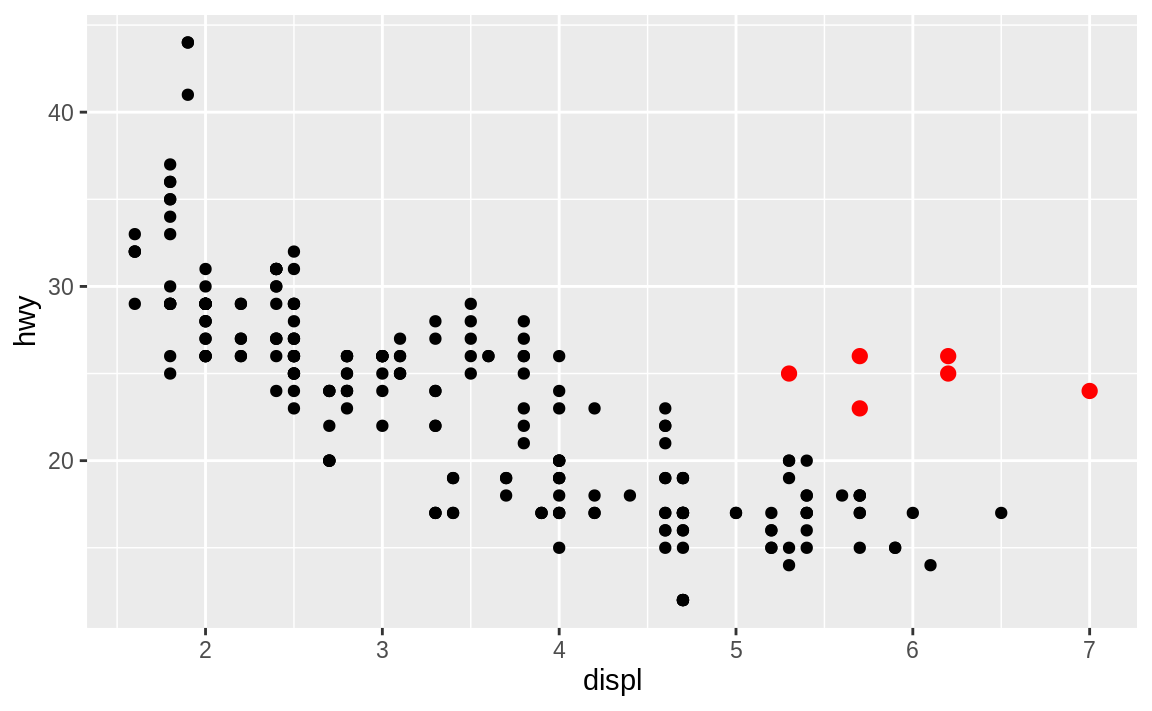
\includegraphics[scale=.5]{figures/outl.png}
\caption{Fuel consumption (Hwy) vs engine size (displ)}
\end{figure}

\end{frame}

% Frame
%--------------------------------------------------------------

\begin{frame}{Multinomial $\land$ Dirichlet model}

Model selection:

\begin{itemize}

\item Likelihood: $\bm{x}|\bm{\theta} \sim \mathcal{M}_k(N,\bm{\theta})$

\item Hypotheses:  $ H_0: \bm{\theta}=\bm{\theta_0} \,\,\,\, \text{vs} \,\,\,\,  H_1: \bm{\theta} \neq \bm{\theta_0}$

\item Prior: $\pi(\bm{\theta}|H_0)={1_{\bm{\theta_0}}(\bm{\theta_0})}$ and $\bm{\theta}|H_1, \bm{\alpha} \sim \operatorname{Dir}_k(\bm{\alpha})$ 

\item Marginal density: $m_i(\bm{x})=\int_{\Theta_i} f(\bm{x}|\bm{\theta})\pi(\bm{\theta}|H_i) \, d\bm{\theta} $, \, $i=0,1$

\begin{itemize}

\item  $m_0(\bm{x})=\frac{N!}{\prod_{i=1}^{k+1}x_i!}\prod_{i=1}^{k+1}{\theta_{0i}}^{x_i}$ 
\item  $m_1(\bm{x})= \frac{N!}{\prod_{i=1}^{k+1}x_i!}\frac{B(\bm{\alpha}+\bm{x})}{B(\bm{\alpha})}$ 

\end{itemize}

\item Bayes factor: $B_{01}(\bm{x}) = \frac{m_0(\bm{x})}{m_1(\bm{x})} = \frac{\prod_{i=1}^{k+1}{(\theta_{0i}}^{x_i}) \prod_{i=1}^{k+1}[\Gamma(\alpha_i)] \Gamma [\sum_{i=1}^{k+1}(\alpha_i+x_i)]}{\Gamma(\sum_{i=1}^{k+1} \alpha_i) \prod_{i=1}^{k+1}\Gamma(\alpha_i+x_i)}$

\item For an interesting application see \citet{pericchiTorres2011}.

\end{itemize}

\end{frame}

% Frame
%--------------------------------------------------------------

\begin{frame}{Multinomial $\land$ Dirichlet model}

Parameter estimation:

\begin{itemize}

\item Prior: $\bm{\theta}|\bm{\alpha} \sim \operatorname{Dir}_k(\bm{\alpha})$

\item Posterior: $\bm{\theta} | \bm{\alpha}, \bm{x} \sim \operatorname{Dir}_k(\bm{\alpha} + \bm{x}) \rightarrow$ Mean, mode, credible intervals.

\item For an interesting application see \citet{ley1996peculiar}.


\end{itemize}

\end{frame}

% Frame
%--------------------------------------------------------------

\begin{frame}{Binomial $\land$ Dirichlet Beta}

Model selection:

\begin{itemize}

\item Likelihood: $x \sim \text{Bin}(N, \theta)$

\item  Hypotheses: $ H_0: {\theta}={\theta_0} \,\,\,\, \text{vs} \,\,\,\,  H_1: {\theta} \neq \theta_0$

\item Prior: $\pi(\theta|H_0)={1_{\theta_0}(\theta)}$ and $\theta| H_1 \sim \operatorname{Beta}($a$,$b$) $

\item Marginal density: $m_i(x)= \int_0^1 f(x|\theta)\pi(\theta|H_i)d \theta, \,  i=0, 1$

\begin{itemize}

\item $m_0(x)=\binom{N}{x} {\theta_0}^{x}{(1-\theta_0)}^{N-x}$ 

\item  $m_1(x) = \binom{N}{x}\frac{B(x+a, n-x+b)}{B(a,b)}$

\end{itemize}

\item Bayes factor: $B_{01}(x) = \frac{m_0(x)}{m_1(x)}  = \frac{\theta_0(1-\theta_0)^{N-x}\,\Gamma(a)\,\Gamma(b)\,\Gamma(n+a+b)}{\Gamma(a+b)\,\Gamma(n+a-x)\,\Gamma(x+a)}$ 

\end{itemize}

\end{frame}

% Frame
%--------------------------------------------------------------

\begin{frame}{Binomial $\land$ Dirichlet Beta}

Parameter estimation:

\begin{itemize}

\item Prior: $\theta \sim \operatorname{Beta}(a,b) $

\item Posterior: $\theta | x \sim \operatorname{Beta}(a+x, b+N-x ) \rightarrow$ Mean, mode, credible intervals

\end{itemize}

\end{frame}

% Frame
%--------------------------------------------------------------

\begin{frame}[fragile]{Python code looks good on verbatim}

This code prints the Fibonacci sequence:

\begin{verbatim}
nterms = int(input("How many terms? "))
n1, n2 = 0, 1
count = 0
print("Fibonacci sequence:")
while count < nterms:
    print(n1)
    nth = n1 + n2
    n1 = n2
    n2 = nth
    count += 1
}
\end{verbatim}

\end{frame}

% Frame
%--------------------------------------------------------------

\begin{frame}[fragile]{Some R code}

I also included a verbatim environment with background color:

\begin{cverbatim}
getmode <- function(v) {
  
  uniqv <- unique(v)
  
  uniqv[which.max(tabulate(match(v, uniqv)))]
  
}
\end{cverbatim}

With this R code you can build a function that calculates the mode.

\end{frame}

% Bibliography page (can be commented out)
%--------------------------------------------------------------

% Code to generate the "references" section
%--------------------------------------------------------------

\section[]{References}
\subsection{}

\begin{frame}[allowframebreaks]{References}
\printbibliography
\end{frame}

% End of the document
%--------------------------------------------------------------
\end{document}















